%Cambio lo stile delle sezioni da numeri a lettere
\renewcommand\thesection{\Alph{section}}
%Imposto come lettera la "O" di Organigramma
\setcounter{section}{14} 
%Colonna per centrare in orizzontale/verticale
\newcolumntype{M}[1]{>{\centering\arraybackslash}m{#1}}
\newsection{Organigramma}

\subsection{Redazione}
\renewcommand{\arraystretch}{2}
\begin{table}[H]
\begin{center}
  \begin{tabular}{| c | c | c |}
    \hline
    \rowcolor{title_row}
    \textbf{\color{title_text}{Nominativo}} & \textbf{\color{title_text}{Data}} & \textbf{\color{title_text}{Firma}} \\ \hline
    Marco Costantino & 30-12-2018 & 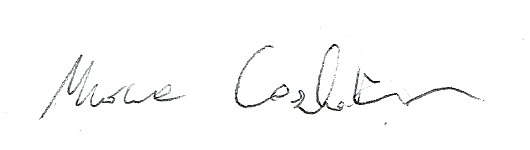
\includegraphics[align=c,scale=1]{Res/Firme/marco.png} \\ \hline
    Michele Roverato & 30-12-2018 & 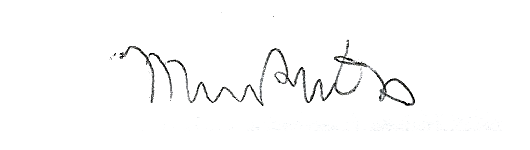
\includegraphics[align=c,scale=1]{Res/Firme/michele.png} \\ \hline
    Nicolò Tartaggia & 30-12-2018 & 
\includegraphics[align=c,scale=1]{Res/Firme/tartizz.png} \\ 
    \hline
  \end{tabular}
  \caption{Tabella O.1: Redazione\label{}}
\end{center}
\end{table}
\renewcommand{\arraystretch}{1}

\subsection{Approvazione}
\renewcommand{\arraystretch}{2}
\begin{table}[H]
\begin{center}
  \begin{tabular}{| c | c | c |}
    \hline
    \rowcolor{title_row}
    \textbf{\color{title_text}{Nominativo}} & \textbf{\color{title_text}{Data}} & \textbf{\color{title_text}{Firma}} \\ \hline
    Giacomo Barzon & 07-01-2019 & 
\includegraphics[align=c,scale=1]{Res/Firme/giacomo.png} \\ \hline
    Tullio Vardanega &  &  \\
    \hline
  \end{tabular}
  \caption{Tabella O.2: Approvazione\label{}}
\end{center}
\end{table}
\renewcommand{\arraystretch}{1}

\subsection{Accettazione dei componenti}
\renewcommand{\arraystretch}{2}
\begin{table}[H]
\begin{center}
  \begin{tabular}{| c | c | c |}
    \hline
    \rowcolor{title_row}
    \textbf{\color{title_text}{Nominativo}} & \textbf{\color{title_text}{Data}} & \textbf{\color{title_text}{Firma}} \\ \hline
    Andrea Trevisin & 07-01-2019 & 
\includegraphics[align=c,scale=1]{Res/Firme/andrea.png} \\ \hline
    Giacomo Barzon & 07-01-2019 & 
\includegraphics[align=c,scale=1]{Res/Firme/giacomo.png} \\ \hline
    Giovanni Sorice & 07-01-2019 & 
\includegraphics[align=c,scale=1]{Res/Firme/ciro.png} \\ \hline
    Lorenzo Busin & 07-01-2019 & 
\includegraphics[align=c,scale=1]{Res/Firme/lorenzo.png} \\ \hline
    Marco Costantino & 07-01-2019 & 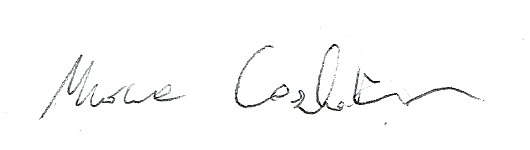
\includegraphics[align=c,scale=1]{Res/Firme/marco.png} \\ \hline
    Michele Roverato & 07-01-2019 & 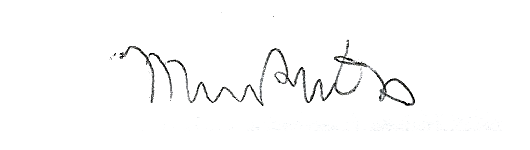
\includegraphics[align=c,scale=1]{Res/Firme/michele.png} \\ \hline
    Nicolò Tartaggia & 07-01-2019 & 
\includegraphics[align=c,scale=1]{Res/Firme/tartizz.png} \\ 
    \hline
  \end{tabular}
  \caption{Tabella O.3: Accettazione dei componenti\label{}}
\end{center}
\end{table}
\renewcommand{\arraystretch}{1}

\subsection{Componenti}
\renewcommand{\arraystretch}{2}
\begin{table}[H]
\begin{center}
  \begin{tabular}{| c | c | c | p{3cm} |}
    \hline
    \rowcolor{title_row}
    \textbf{\color{title_text}{Nominativo}} & \textbf{\color{title_text}{Matricola}} & \textbf{\color{title_text}{Email}} \\ \hline
    Andrea Trevisin & 1144684 & andrea.trevisin@studenti.unipd.it \\ \hline
    Giacomo Barzon & 1143164 & giacomo.barzon.2@studenti.unipd.it \\ \hline
    Giovanni Sorice & 1144588 & giovanni.sorice@studenti.unipd.it \\ \hline
    Lorenzo Busin & 1143782 & lorenzo.busin@studenti.unipd.it \\ \hline
    Marco Costantino & 1144120 & marco.costantino@studenti.unipd.it \\ \hline
    Michele Roverato & 1143030 & michele.roverato.2@studenti.unipd.it \\ \hline
    Nicolò Tartaggia & 1142836 & nicolo.tartaggia@studenti.unipd.it \\ 
    \hline
  \end{tabular}
  \caption{Tabella O.4: Lista Componenti\label{}}
\end{center}
\end{table}
\renewcommand{\arraystretch}{1}
\pagebreak